
\section{Server Overview}

In order to negotiate the connection setup between two or more clients, we decided to
design and implement a server application. The server 
manages the clients' connection statuses, similar to an instant messaging
server.
It provides a method for clients to sign on or off, a way to check friends' online
statuses, and a method to request a friend's ip address and port.

\subsection{Server Design Decisions}

We had to make a number of design decisions for the server, which are described here.

We'll start with the choice of implementation language. Because the server is a
separate entity from the chat client, we had some extra freedom for language and
design choice. The primary requirement for the server was that it must be able
to connect and communicate with each client. After some consideration, we
implemented the server in Python for two main reasons. First, Python
has a number of modules, including a socket-based asynchronous server, available
to aid with development. Second, Python's general syntax and ease of use makes
it a great tool for creating mock-ups or relatively small, short-term projects.
Of course, it works well for larger projects too. Python made coding much
cleaner and more maintainable for the goals of our project.

We wanted the server to perform some of the same capabilities that a
watered-down chat server (such as one used for Skype) might have or use. To that
end, we needed it to have login functionality and user tracking. We determined
that the server had to perform the following tasks at minimum.

\begin{enumerate}
  \item Provide a way for a user to register that he or she is online.
  \item Provide a way for users to talk to each other.
  \item Maintain a list of users each client is permitted to contact.
  \item Provide information updates to each user about their friends' online statuses.
\end{enumerate}

The first task is essential because it represents the core reason for adding a
server element: to keep track of users. By giving users a way to register that
they are connected (and conversely, allow them to disconnect as needed), the
server could keep track of users as they log in or log out, allowing it to
perform additional functionality. This is also required for task 4 and is the
basis of the notification system on the client side.

The second task is important because users shouldn't be expected to know the IP
address or port number of the computers their friends are on. The client needs a
way of obtaining this information from the server, and thus being able to chat
with others. It is important that this information be maintained by the server
so that users have more freedom when using our system. When testing, it also
provided the benefit of not needing to manually enter in a new IP address/port
number combination every time we want to initiate a chat session. The main
drawback for this feature is that a client must request for this information
every time he or she wants to start a chatting session with one of his or her
friends.

Strictly speaking, only points 1 and 2 above are actually needed for a
minimalistic server to function. The server keeps track of who is online, and
tells clients where they can contact other clients who are online. However, we
wanted our server to emulate some additional features seen in commercial media
streaming applications. This leads to our third task: maintaining a friends list
for each client.
The server keeps a list of who is friends with whom, thereby limiting clients from being able to randomly call or spam other users who might be online.

The final task is fairly closely related to task 3. In order to cache friend
information on the client side (so the client won't make chat requests for
offline users), the server should be capable of periodically sending updates to
each connected client. These updates notify the client of which of his friends
he is able to call at any given time.

Our final core design choice relates to storage of user information. As it is
standard in industry, we decided the server should store information in a
database file that is easily accessible without any parsing or configurations.
In this database, the server would keep track of user and friend list
information, as well as any other necessary information needed, i.e. IP
addresses and port numbers. Although it isn't very much information to keep
track of, it still gives a relatively simple solution to keeping track of users
without the overhead of having to store information manually (such as in a text
file).
 
\subsection{Server Implementation}
Now that we've covered the key design decisions of the server, we will describe how the server
was implemented. A generalized state diagram is shown in Fig.~\ref{fig:server_diag}.

\begin{figure*}[!t]
   \centering
      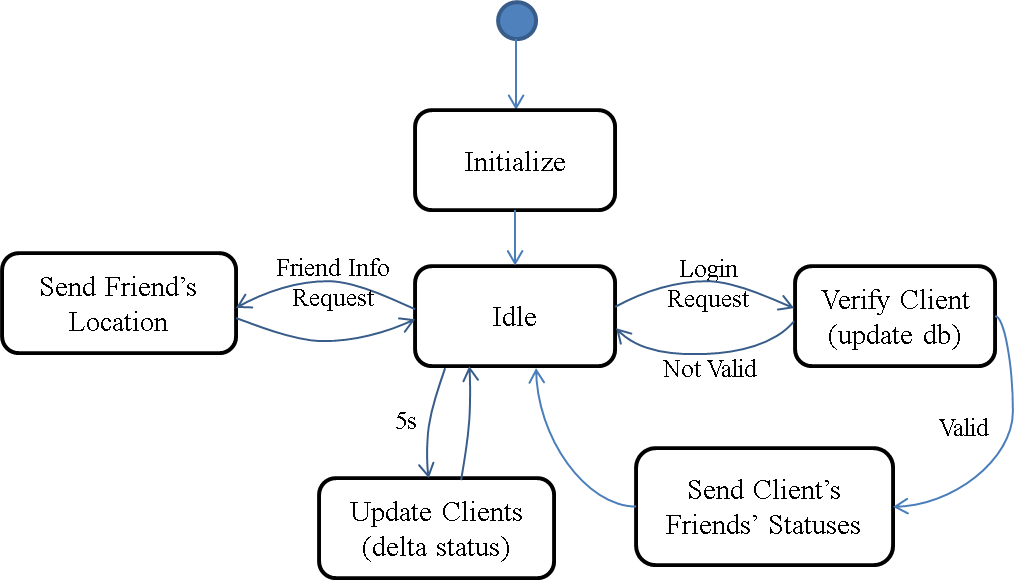
\includegraphics[width=0.8\textwidth]{pics/Server_StateDiagram2}
   \caption{Server State Diagram demonstrating the general flow of the central server.}
\label{fig:server_diag}
\end{figure*}


Python has a number of different modules available for applications to communicate
through using network sockets. Our first consideration was the SocketServer module. This 
library
provides an interface which can block receive requests, and then execute a request
handler via a callback. Unfortunately, this module has one major flaw: it can only handle
one user request at a time. Because the server needed to handle multiple connected users
asynchronously, we settled on using the asyncore module. This module has essentially
the same functionality as SocketServer, but with asynchronous I/O and support for multiple clients. With this module, each
new incoming connection request from a client executes a request handler in its own seperate thread, allowing 
multiple clients to connect and remain logged in at the same time.

To allow clients to log on, request information, and receive updates, it made
sense for the server to use a reliable connection-oriented protocol. Thus, TCP was the 
natural
choice for client to server communication. When a client connects to the server, the server spawns a new thread to maintain
the connection to the client. If the client makes any requests, the response packets will 
be sent
directly to the child thread connected to that client instead of the main server loop. Each child thread has its own
instance of a request handler that controls the logic for reading, interpreting, and replying
to each client request. If a client closes its connection, the thread closes as well and is
removed from the loop. 

To log in, a client establishes a connection to the server (in our tests
the client would accept the IP address of the server as an input parameter) and sends it
a packet with two 20 byte strings: a username and a password, padded as necessary with
null bytes. The server then accepts the packet, verifies the username and password, and
replies back to the client with either a success or failure packet depending on the
validity of the credentials. The password is sent over the network as plaintext (normally
it would be encapsulated in an SSL connection) and the server, upon reception, hashes
the password with a salt using an SHA-512 function and compares the result to the stored hash value 
in the database. If the hashes match, the user is granted login privileges. This
security isn't hack-proof, but it at least models a standard login procedure.  Additional
security concerns are left for future work.

Once a client successfully logs in, the server replies back with a friend list packet.
This packet contains a list of usernames and IDs for all the client's current
friends.
This packet does not contain any online statuses, and in the event of an overflow (more friends than can fit in the packet) the server would simply truncate
the list. We did not run into any issues with this in testing because we only had 2
users, but in a real-world environment this certainly would be more of a concern and 
therefore is left for future work.

Every few seconds (our implementation configured it to 4), the server sends out an
update to each client currently maintaining a connection to it. To accomplish this,
the server initializes a timer to provide an interrupt which executes a special method
once per interval. This method, when run, determines who has changed status in the past
interval (whether they went online or offline), and sends each of the clients' friends a 
status update. To reduce the overhead of using the same
connection, this status update would be sent via a separate connection that each client
establishes when it first connects. When the method finishes executing, it uses a callback
to set up a new timer interrupt. 

One other capability the server provides to each client is a friend address request. Due to
the nature of our project and the desire to avoid repeatedly entering IP
addresses and port information
when performing tests, we implemented the ability for a client to request a friend's IP 
address and port number
information from the server. A client simply sends a packet containing the
friend's ID. The server, upon verifying the friend is indeed a friend and is
online, replies with the IP address and the port number of that friend's computer. This information is then used
by the client to establish a client-to-client connection that is independent of the 
server. Because we did not desire an intermediary machine, we chose not to route client to client
communication through the server itself.

For sending and receiving binary data over the network, the server uses the Python struct
module, which provides a convenient way to pack and unpack data with specific size
limits. When sending data, the server calculates the values it needs, packs them as
appropriate, and concatenates the values together (the struct module uses strings
for its binary representation, in which an encoded character represents the specific values
we want to send or receive). When receiving data, the server decodes a character
to identify the type of packet received.

To keep track of users and friends, the server uses a SQLite database consisting of
two tables. The first table, called ``Users,'' has one row per user, with columns
giving the username, user ID, and password hash. The second table, called ``Friends,''
contains a row per user which includes each of the users friends. The design of this is such
that ``A is friends with B'' and ``B is friends with A'' needs to occur in the table
for A and B to properly communicate. In other words, for every set of friends, two rows
in the ``Friends'' table are needed. This is not exactly the most efficient (or even the
most reliable) way to keep track of the information, but the implementation served well enough
for the scope of this project. When the server wants to obtain information from the
database, it uses the sqlite3 Python module to do so. 
